% !TeX root = ../../main.tex
\section{Introduction}
%he development of a continuous process for the nitration process of toluene into nitrotoluene has been
This report aims to design a feasible and optimised reactor for the production of o-toluidine, 4-aminobenzaldehyde and 4-aminobenzoic acid. The two (?) major challenges in this reactor design are namely:
\begin{enumerate}
    \item The safety risk of a highly exothermic nitration process of converting toluene into nitrotoluene and to ensure an inherently safer continuous nitration process. 
    \item Transitioning away from a batch process which was mainly used in similar fine chemicals manufacture, into continuous process. 
\end{enumerate}



%Include COMSOL and mechanically design on AutoCAD

\textcolor{red}{include overall chemdraw diagram here} %or should the reactor PNID or block flow diagram be better? doesnt really show the R101 etc names in this diagram
\subsection{Reactors overview}
\begin{figure}[h]
    \centering
    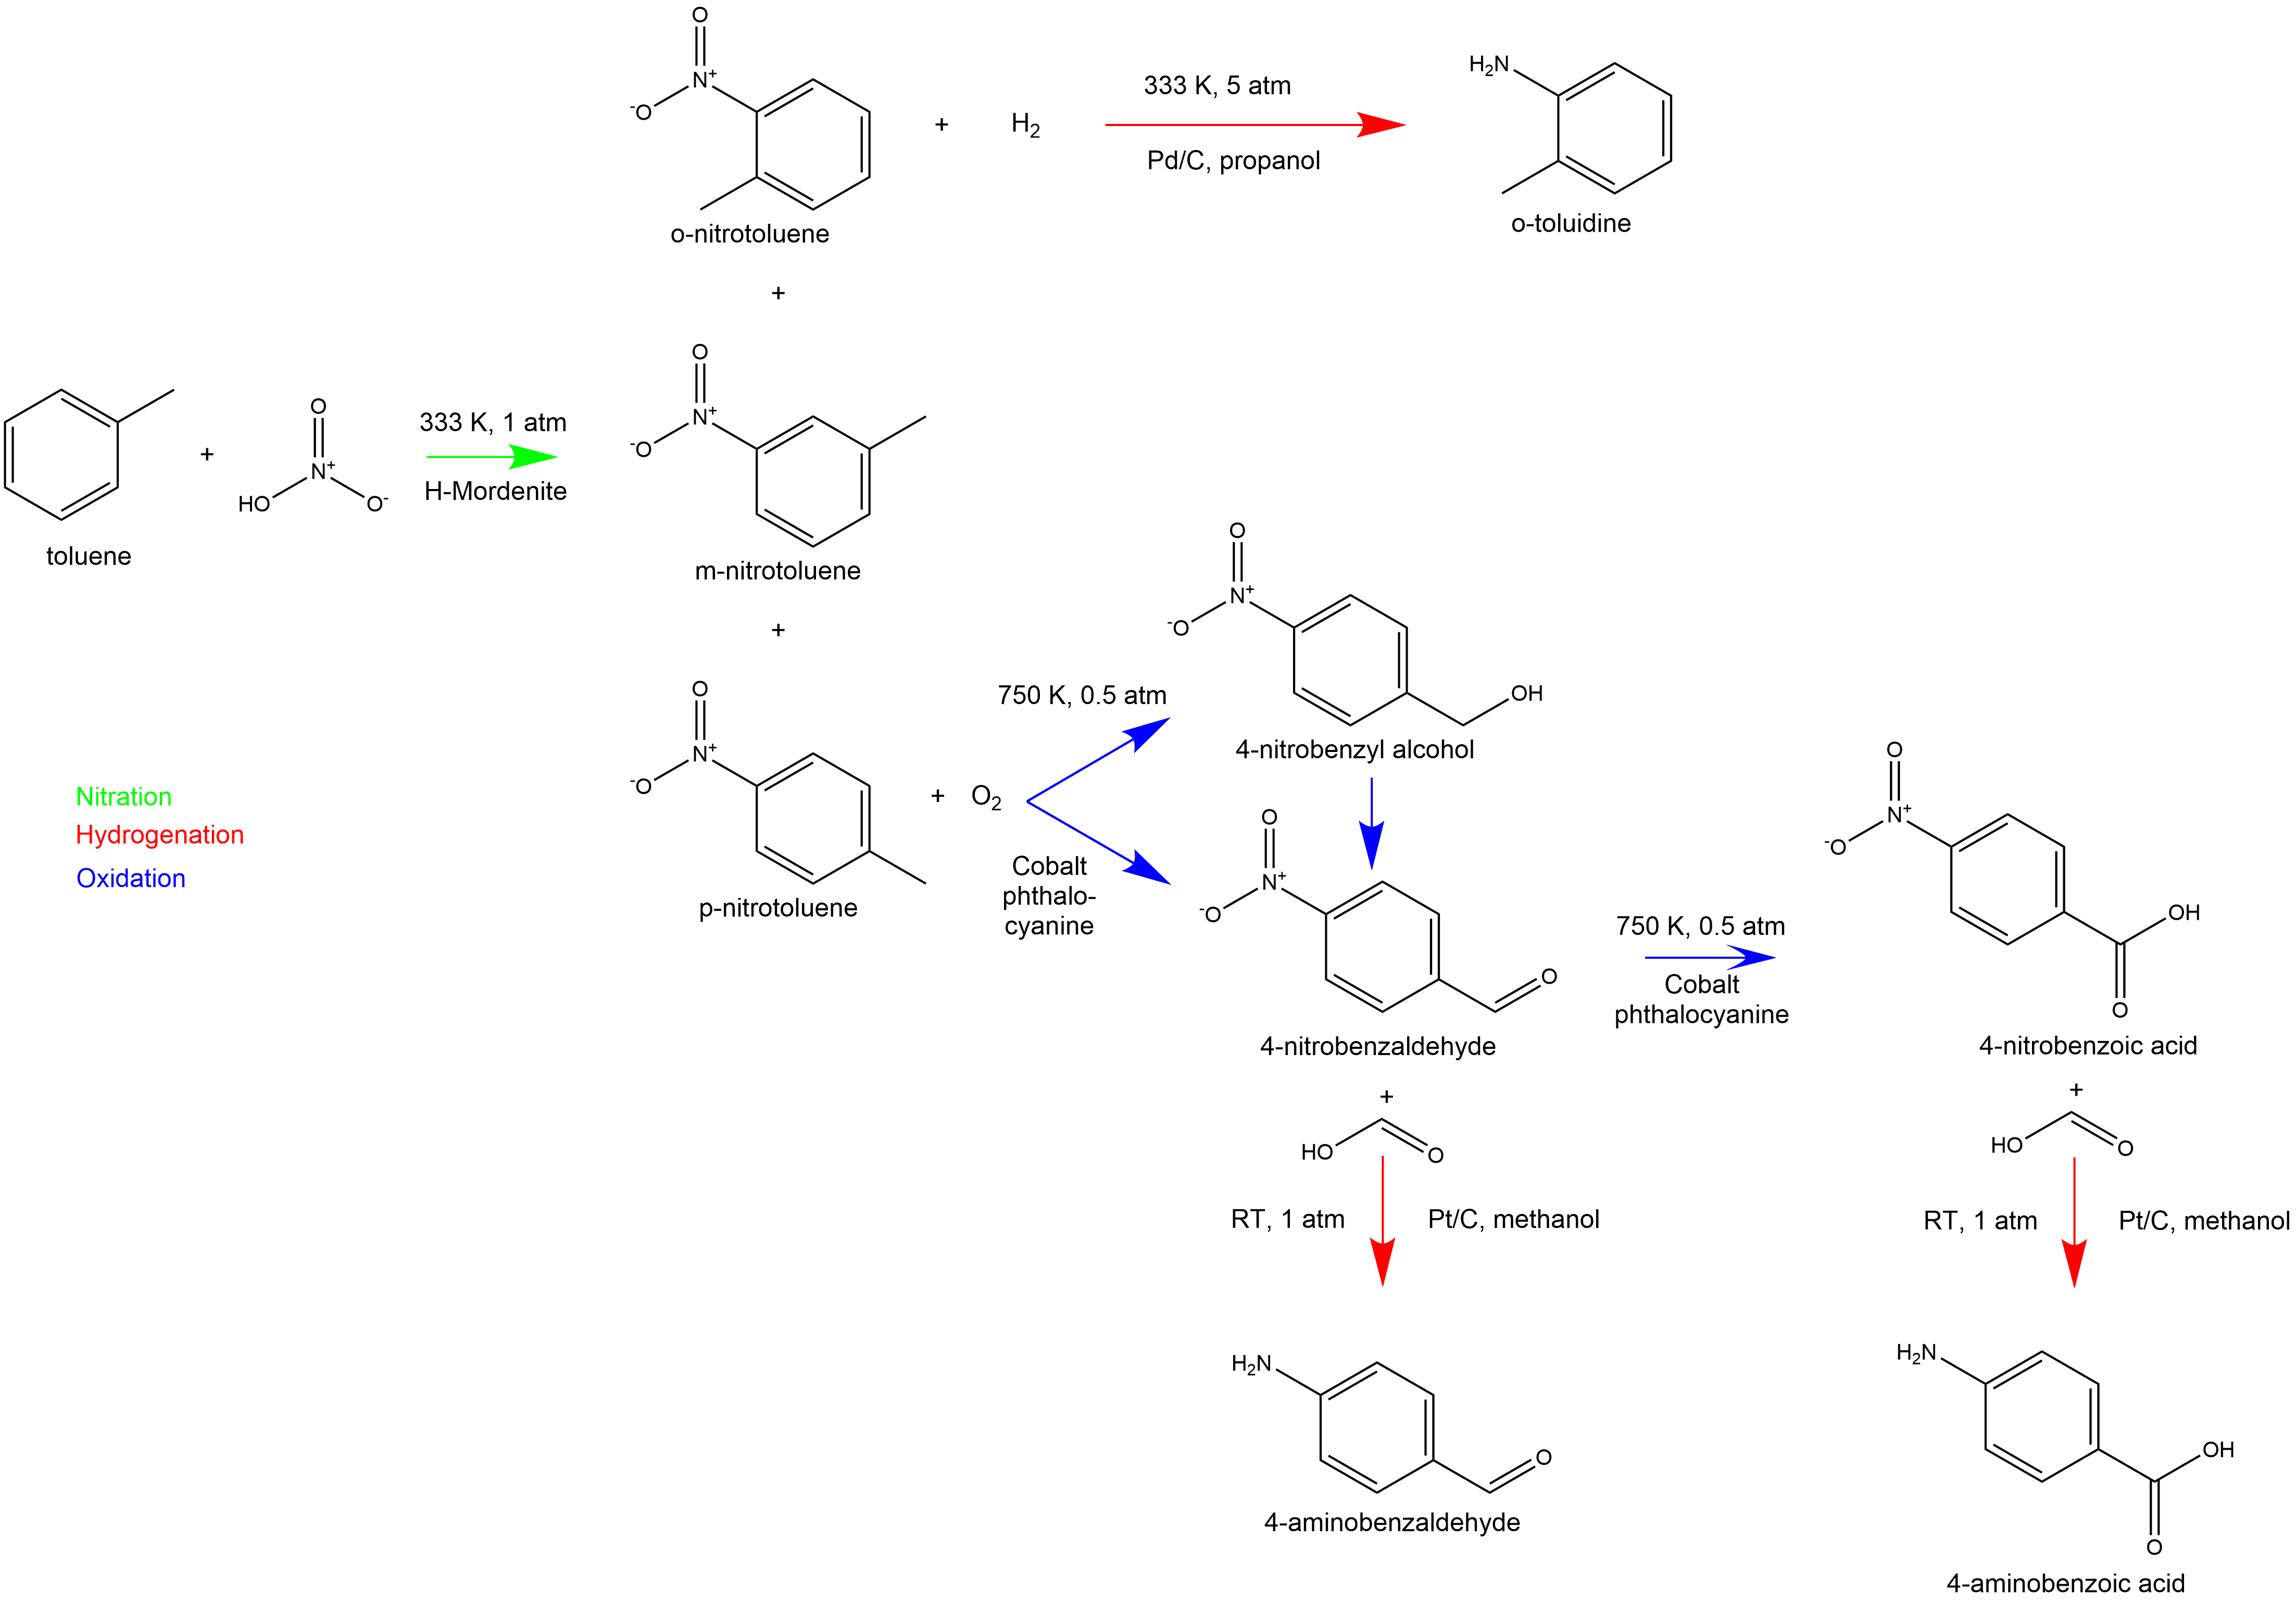
\includegraphics[width=\linewidth]{chapters/2-reaction/figures/routes-chosen_20210220.png}
    \caption{Reaction scheme proposed by Nitroma}
    \label{fig:finalroutes}
\end{figure}
Figure \ref{fig:finalroutes} denotes the proposed overall reaction scheme of Nitroma's process. The first reactor R101 is an intensified shell-and-tube heat exchanger reactors, used for the nitration of toluene to produce isomers ortho-nitrotoluene (ONT), meta-nitrotoluene (MNT) and para-nitrotoluene (PNT). Next, reactor R201 is a co-current trickle bed reactor that enables the ONT to be hydrogenated into o-toluidine in methanol solvent. Packed-bed reactors R301 and R302 are used for the oxidation of PNT into p-nitrobenzaldehyde (pNBH) and p-nitrobenzoic acid (pNBA) production respectively. Finally, both pNBH and pNBA are hydrogenated into p-aminobenzaldehyde and p-aminobenzoic acid in packed-bed reactors R401 and R501 respectively. Further details on how each reactors were chosen are detailed in Section \ref{Non-detailed}. 

\textcolor{red}{Double confirm the remaining reactors (it was microreactor previously)} 

%Things to double check!
%-sequence of subsections (group by dimension/heat transfer mass transfer?)
%-storyline of reactor? what final KPI should we be looking at?



